\documentclass{article}
\usepackage{fullpage}
\usepackage{graphicx}
\usepackage{amsmath}
\usepackage{mathtools}
\usepackage{xcolor}
\usepackage{bm}

\usepackage{natbib}
\usepackage[hidelinks]{hyperref}
\usepackage{doi}
\usepackage{charter}
\usepackage[bitstream-charter]{mathdesign}
\usepackage[final,babel]{microtype}
\usepackage[utf8]{inputenc}
\usepackage[british]{babel}
\usepackage{csquotes}
\usepackage[T1]{fontenc}
\usepackage{siunitx}


\title{Multidimensional advection over steep terrain on a new type of Cartesian mesh \\ \TODO{(working title)}}
\author{James Shaw}

\newcommand{\iunit}{\boldsymbol{\hat \imath}}
\newcommand{\junit}{\boldsymbol{\hat \jmath}}
\newcommand{\kunit}{\boldsymbol{\hat k}}
\newcommand{\TODO}[1]{\textcolor{purple}{TODO: \emph{#1}}}

\begin{document}
\maketitle

\section{Introduction}

First, we present a multidimensional advection scheme that is computationally cheap and suitable for complex flows on arbitrary meshes.  Second, we present a new type of Cartesian mesh, the slanted cell mesh, that avoids the small cell problem associated with cut cell meshes.   We apply the advection scheme to tests over steep orography and show that accurate results are obtained on slanted cell meshes.  Finally, we challenge the multidimensional advection scheme using a test of deformational flow on a geodesic mesh.

\section{Slanted cell mesh generation}

\begin{figure}
	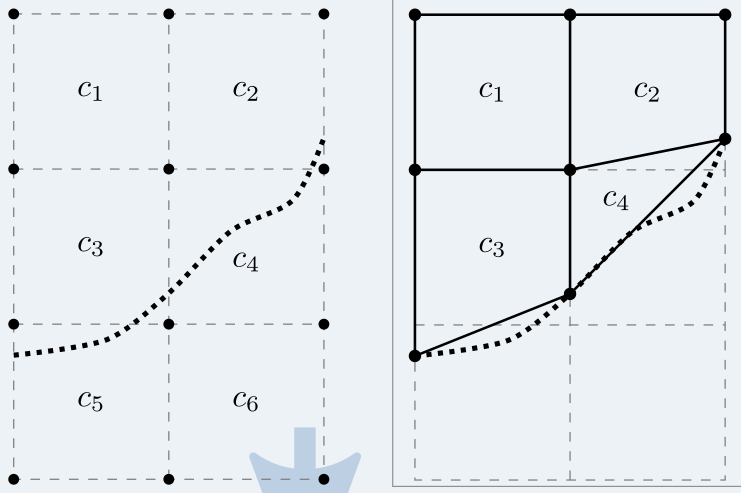
\includegraphics[width=0.5\textwidth]{slantCellConstruction.png}
	\caption{\TODO{Before and after diagrams showing how a slanted cell mesh is constructed from a uniform quadrilateral mesh}}
\end{figure}

\begin{figure}
	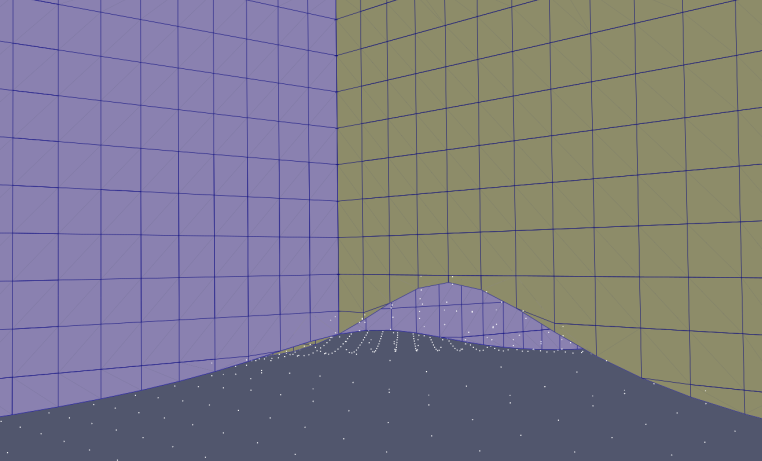
\includegraphics[width=0.5\textwidth]{3dslices.png}
	\caption{\TODO{An example of a 3D slanted cell mesh with Alpine topography, maybe best illustrated using orthogonal cross-sections.  Can we show this for triangles, quads and hexagons?}}
\end{figure}

\begin{figure}
	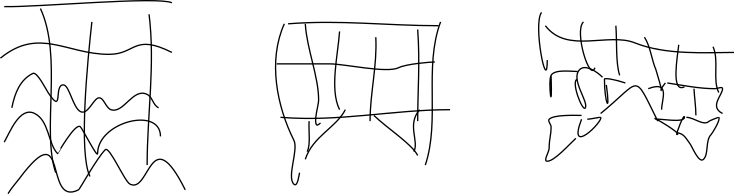
\includegraphics[width=\textwidth]{meshComparison.png}
	\caption{\TODO{examples of BTF, slanted cell and cut cell meshes with the same steep mountain profile (one of those used in the thermal advection test)}}
\end{figure}

\clearpage

\section{Multidimensional advection scheme}

The advection of a dependent variable $\phi$ is given by the flux form conservation equation:
\begin{align}
	\frac{\partial \phi}{\partial t} + \nabla \cdot \left( \bm{u} \phi \right) = 0 \label{eqn:advection}
\end{align}
where $\bm{u}$ is a prescribed wind field.  The time derivative is discretised using a three-stage, second-order Runge-Kutta scheme:
\begin{subequations}
\begin{align}
	\phi^\star &= \phi^{(n)} + \Delta t f(\phi^{(n)}) \\
	\phi^{\star\star} &= \phi^{(n)} + \frac{\Delta t}{2} \left( f(\phi^{(n)}) + f(\phi^\star) \right) \\
	\phi^{(n+1)} &= \phi^{(n)} + \frac{\Delta t}{2} \left( f(\phi^{(n)}) + f(\phi^{\star\star}) \right)
\end{align}
\end{subequations}
where \(f(\phi^{(n)}) = - \nabla \cdot (\bm{u} \phi^{(n)})\) at time level \(n\).

Using the finite volume method, the wind field is prescribed at face centroids and the dependent variable is stored at cell centroids.  The divergence term in equation~\eqref{eqn:advection} is discretised using Gauss's theorem:
\begin{align}
	\nabla \cdot \left( \bm{u} \phi \right) \approx \frac{1}{\mathcal{V}_c} \sum_{f \in c} \bm{u}_f \cdot \bm{S}_f \phi_F
\end{align}
where $\mathcal{V}_c$ is the cell volume, $\bm{u}_f$ is a wind vector prescribed at a face, ${\bm{S}_f}$ is the surface area vector with a direction outward normal to the face and a magnitude equal to the face area, and $\sum_{f \in c}$ denotes a summation over all faces $f$ belonging to cell $c$.  The value of the dependent variable at the face, $\phi_F$, is approximated by a least squares fit over a stencil of surrounding cell centre values.

\begin{figure}
	\centering
	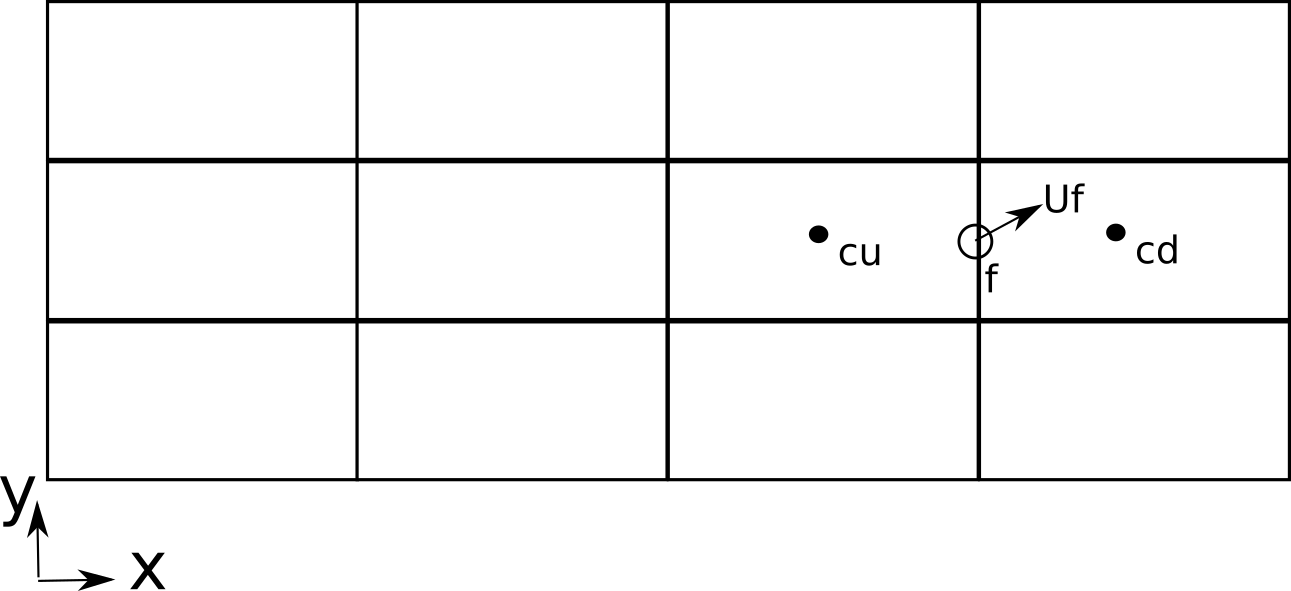
\includegraphics[width=4in]{interiorQuadStencil.png}
	\caption{\TODO{interior quad stencil}}
	\label{fig:interiorQuadStencil}
\end{figure}

To introduce the approximation method, we will consider how an approximate value is calculated for a face in the interior of a two-dimensional uniform quadrilateral mesh.  For any mesh, every interior face connects two adjacent cells.  The wind direction at the face determines which of the two adjacent cells is the upwind cell.  Since the stencil is upwind-biased, two stencils must be constructed for every interior face, and the appropriate stencil is chosen for each face depending on the wind direction at that face for every timestep.

The upwind-biased stencil for a face $f$ is shown in figure~\ref{fig:interiorQuadStencil}.  The wind at the face, $\bm{U}_f$, is blowing from the upwind cell $c_u$ to the downwind cell $c_d$.
To obtain an approximate value at $f$, a polynomial least squares fit is calculated using the stencil values.
The stencil has \num{4} points in $x$ and \num{3} points in $y$, leading to a natural choice of polynomial that is cubic in $x$ and quadratic in $y$:
\begin{align}
	\phi = a_1 + a_2 x + a_3 y + a_4 x^2 + a_5 xy + a_6 y^2 + a_7 x^3 + a_8 x^2 y + a_9 x y^2
\end{align}
A least squares approach is needed because the system of equations is overdetermined, with \num{12} stencil values but only \num{9} polynomial terms.  If the stencil geometry is expressed in a local coordinate system with the face centroid as the origin, then the approximated value $\phi_F$ is equal to the constant term $a_1$.

The remainder of this section generalises the the approximation technique for arbitrary meshes, explaining the methods for constructing stencils, choosing the terms of the polynomial, and ensuring numerical stability of the advection scheme.


\subsection{Stencil construction}

\subsection{Polynomial generation}
% generating candidates
% full rank check

\subsection{Stabilisation procedure}
% stability constraints
% reweighting

Stability constriants:
\begin{align}
	0.5 \leq u \leq 1 \\
	0 \leq d \leq 0.5 \\
	u - d \geq \max(|p|)
\end{align}

\begin{figure}
	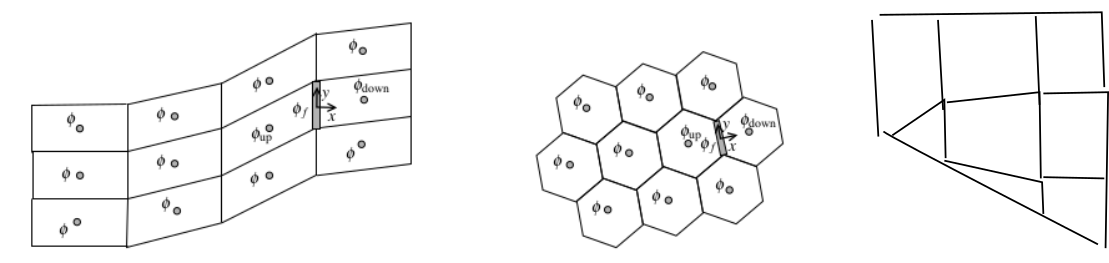
\includegraphics[width=\textwidth]{stencilConstruction.png}
	\caption{\TODO{example stencils in interior of quad and hex meshes, and example stencil near boundary of a slanted cell mesh (taken from one of the test cases)}}
\end{figure}


\section{Results}
\subsection{\TODO{Horizontal advection?}}

\subsection{Thermal advection}

Domain \SI{301}{\kilo\meter} wide, \SI{25}{\kilo\meter} high, Sch\"ar had $\Delta x = \SI{1}{\kilo\meter}, \Delta z^\star = \SI{500}{\meter}$.  Integrate \SI{18000}{\second} so that tracer initially at left hand edge of mountain has safely passed through the outlet boundary (i.e. we are in a steady-state solution).  $\Delta t = \SI{25}{\second}$ for Sch\"ar's mesh.

\begin{table}
	\begin{verbatim}
61x10		5000
121x20		2500
151x25		2000
241x40		1250
301x50		1000
451x75		 667
601x100		 500
901x150		 333
1201x200	 250
2401x400	 125
3001x500	 100
	\end{verbatim}
	\caption{\TODO{suggested $x$ cells $\times$ $z$ cells $\times \Delta t$ resolutions for thermal advection convergence tests}}
\end{table}

Mountain profile:
\begin{subequations}
\begin{align}
   h(x) &= h^\star \cos^2 ( \alpha x )
%
\intertext{where}
%
   h^\star(x) &= \left\{ \begin{array}{l l}
       h_0 \cos^2 ( \beta x ) & \quad \text{if $| x | < a$} \\
	0 & \quad \text{otherwise}
    \end{array} \right.
\end{align}
\end{subequations}
where $a = \SI{25}{\kilo\meter}$ is the mountain envelope half-width, $h_0 = \SI{6}{\kilo\meter}$ is the maximum mountain height, $\lambda = \SI{8}{\kilo\meter}$ is the wavelength, \(\alpha = \pi / \lambda\) and \(\beta = \pi / (2a)\).

$h0, a$ and $\lambda$ are chosen to give us very steep terrain, and to match those from Hilary and Yumeng's upcoming QJRMS paper.

Initial thermal profile:
\begin{align}
	\theta(z) = \theta_0 \exp \left( \frac{N^2}{g} z \right) \label{eqn:thermal-profile}
\end{align}

Velocity field:
\begin{equation}
	\Psi(x,z) = -u_0 H \frac{z - h}{H - h} \label{eqn:streamfunc-btf}
\end{equation}
where $u_0 = \SI{10}{\meter\per\second}$, which is the horizontal wind speed where $h(x) = 0$.
The horizontal and vertical components of velocity, $u$ and $w$, are then given by
\begin{align}
	u &= -\frac{\partial \Psi}{\partial z} = u_0 \frac{H}{H - h}, \quad w = \frac{\partial \Psi}{\partial x} = u_0 H \frac{\mathrm{d} h}{\mathrm{d} x} \frac{H - z}{\left( H - h \right)^2} \label{eqn:uw-btf} \\
	\frac{\mathrm{d} h}{\mathrm{d} x} &= - h_0 \left[ 
		\beta \cos^2 \left( \alpha x \right) \sin \left( 2 \beta x \right) +
		\alpha \cos^2 \left( \beta x \right) \sin \left( 2 \alpha x \right)
	\right]
\end{align}

Analytic solution:
\begin{align}
	\theta_T(x, z) = \theta_0 \exp \left( \frac{N^2}{g} z^\star(x, z) \right) 
\end{align}

\begin{figure}
	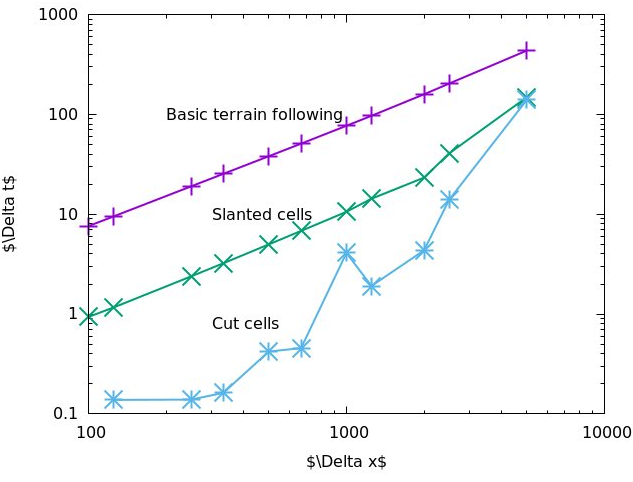
\includegraphics[width=\textwidth]{maxTimesteps.png}
	\caption{\TODO{maximum timesteps (Co=1) for BTF, slanted cells and cut cells: BTF and slanted cells scale linearly with mesh spacing, cut cells do not}}
\end{figure}

\begin{figure}
	\caption{\TODO{error fields for BTF, slanted cells and cut cells at a given mesh spacing, showing errors generated over slopes and advected downstream on slanted cell and cut cell meshes}}
\end{figure}

\begin{figure}
	\includegraphics{../fig-thermalAdvection-convergence/fig-thermalAdvection-convergence.pdf}
	\caption{\TODO{thermal advection l2 and linf convergence plots comparing BTF, slanted cells and cut cells, cubicUpwindCPCFit and linearUpwind}}
\end{figure}

\subsection{Resting atmosphere over Alpine terrain}

\subsection{Deformational flow}
Following \citep{lauritzen2012}.  \TODO{which of the initial conditions should I use?  slotted cylinder would be the hardest}

\section{Conclusions}

The slanted cell method
\begin{itemize}
	\item alleviates the small cell problem
	\item has a linear relationship between mesh spacing and maximum timestep because arbitrarily small cells are not created
	\item accurately represents a hydrostatically balanced atmosphere at rest over steep Alpine terrain
	\item is straightforward to construct compared to the cut cell method
	\item generalises to 3D, applicable to any horizontal mesh structure
\end{itemize}

The advection scheme is
\begin{itemize}
	\item suitable for complex flows on arbitrary meshes
	\item computationally cheap at runtime, with more expensive computations depending only on the mesh geometry
	\item fourth-order convergent at best, first-order convergent at worst
	\item stable for Courant numbers up to 1
\end{itemize}

Idealised atmospheric flows over steep slopes are accurately represented using the multidimensional advection scheme without severely constraining the timestep.  The multidimensional advection scheme is suitable for complex flows on arbitrary meshes.

\section{Acknowledgements}
\TODO{Supervisors, funding bodies.  ASAM group for the mesh generator---I should ask permission to use cut cell meshes in this paper.  Shing Hing Man.}

\bibliographystyle{ametsoc2014}
\bibliography{references}

\end{document}
